\chapter{P2P Systems}\label{chap:p2p}
\gls{p2p} systems represent a paradigm shift in the design and implementation of distributed systems.
In other words, \gls{p2p} systems are decentralized networks where each participant, referred to as a peer, can act as both a client and a server (referred also as servant).
By distributing control and resources among all participating nodes, \gls{p2p} systems overcome many limitations of traditional client-server models.
Unlike the latter, P2P systems leverage the computing power and resources of all the nodes in the network, enabling more scalable and resilient architectures.

\section{Characteristics of P2P Systems}
The decentralized nature of \gls{p2p} systems eliminates the need for a central coordinating authority, which distinguishes \gls{p2p} systems from traditional client-server models.
In a \gls{p2p} network, every node can initiate or respond to requests, share resources, and contribute to the network's overall functionality, leading to important following characteristics.

Decentralization is one of the most fundamental attributes of \gls{p2p} systems.
In these networks, there is no single point of failure or control, which enhances the robustness and resilience of the system.
Each peer operates independently, yet cooperatively, participating in the collective maintenance of the network.
This independence ensures that the failure of a single node or a group of nodes does not damage the entire network, making \gls{p2p} systems highly fault-tolerant (\cite{singh2020}).

Scalability is another significant characteristic of \gls{p2p} systems.
As more peers join the network, the total capacity and available resources increase proportionally.
This growth is organic and does not require significant reconfiguration or central administration.
In structured \gls{p2p} systems, scalability is further enhanced by algorithms such as \glspl{dht}, which ensure that data storage and retrieval operations scale logarithmically with the number of nodes, allowing the network to handle large numbers of peers efficiently (\cite{singh2020}).

Reliability in \gls{p2p} systems is achieved through redundancy and distribution.
Data and resources are typically replicated across multiple nodes, ensuring that the failure of one or more peers does not result in data loss or service interruption.
This redundancy, combined with the system's ability to dynamically reconfigure and redistribute load, contributes to the high availability and reliability of \gls{p2p} networks.
Structured \gls{p2p} systems, like Chord, maintain consistent data access and integrity through well-defined algorithms that handle node join and leave operations gracefully (\cite{stoica2001,zarrin2017}).
The Chord protocol will be discussed in more detail in the Chapter \ref{chap:chord}.

Resource sharing is an inherent characteristic of \gls{p2p} systems, where each peer contributes its own resources, such as bandwidth, storage, and computing power, to the network.
This sharing mechanism leads to a more efficient utilization of available resources compared to traditional systems.
In file-sharing networks, for instance, data is divided into smaller chunks, which are distributed among multiple peers.
This division allows simultaneous downloading and uploading, significantly improving transfer speeds and reducing the load on any single peer (\cite{cohen2003incentives}).

Transparency in \gls{p2p} systems refers to the user's ability to interact with the network without needing to understand its underlying complexities.
\gls{p2p} applications are designed to provide a seamless user experience, where the intricacies of peer connections, data routing, and resource allocation are abstracted away.
Users can access, share, and retrieve resources as if they were interacting with a centralized service, while the \gls{p2p} infrastructure operates in the background to manage these tasks efficiently.

The security of \gls{p2p} systems presents both challenges and advantages.
The decentralized nature reduces the risk of centralized attacks, but it also introduces vulnerabilities such as Sybil attacks, where an adversary generates multiple identities to gain disproportionate influence (\cite{Douceur2002}).
Effective security measures, such as cryptographic techniques, reputation systems, and robust algorithms for identity verification, are crucial for maintaining the integrity and trustworthiness of \gls{p2p} networks.

\section{Types of \gls{p2p} Networks}
There are two types of overlay networks: structured and unstructured.
These networks and their differences are described below.
\subsection{Unstructured \gls{p2p} Networks}
In unstructured \gls{p2p} systems, peers are connected arbitrarily.
There is no fixed topology, and the network is highly dynamic.
Peers join and leave the network frequently, and the connections between them are established randomly.
These systems are characterized by their simplicity and robustness against node failures.
However, they are less efficient in resource discovery compared to structured \gls{p2p} networks.

In unstructured \gls{p2p} systems, peers join the network by connecting to a subset of existing peers.
Each peer maintains a list of neighboring peers, forming a mesh-like topology.
When a peer wishes to find a resource, it broadcasts a query to its neighbors, who forward the query to their neighbors, and so on, until the resource is found or the query's \gls{ttl} expires.
Although unstructured \gls{p2p} systems do not typically employ hashing for data placement, we can model the network's growth and the propagation of queries using probabilistic methods.
For example, if each peer forwards a query to $k$ neighbors, the total number of peers queried after $t$ hops can be approximated by:
\[ N(t) = k^t \]
where $N(t)$ is the number of peers queried, and $k$ is the average number of neighbors each peer forwards the query to.
This exponential growth illustrates the flooding nature of query propagation in unstructured networks (\cite{singh2020}).

Fig. \ref{fig:gnutella} illustrates Gnutella, a classic example of an unstructured P2P network.
In Gnutella, each peer maintains a list of its neighbors and sends query messages to them.
If a neighbor has the requested resource, it responds; otherwise, it forwards the query to its own neighbors.
This flooding mechanism continues until the resource is found or the query's \gls{ttl} expires.
\begin{figure}[htbp]
    \centering
    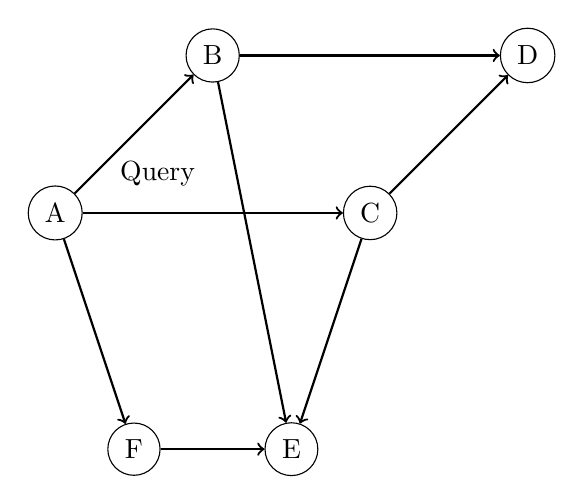
\begin{tikzpicture}
        \node[draw, circle] (A) at (0,0) {A};
        \node[draw, circle] (B) at (2,2) {B};
        \node[draw, circle] (C) at (4,0) {C};
        \node[draw, circle] (D) at (6,2) {D};
        \node[draw, circle] (E) at (3,-3) {E};
        \node[draw, circle] (F) at (1,-3) {F};
      
        \draw[->, thick] (A) -- (B);
        \draw[->, thick] (A) -- (C);
        \draw[->, thick] (B) -- (D);
        \draw[->, thick] (C) -- (D);
        \draw[->, thick] (B) -- (E);
        \draw[->, thick] (C) -- (E);
        \draw[->, thick] (A) -- (F);
        \draw[->, thick] (F) -- (E);
      
        \node at (1.3, 0.5) {Query};
      \end{tikzpicture}
    \caption{Gnutella, an example of unstructured \gls{p2p} network}
    \label{fig:gnutella}
\end{figure}

In this example, peer $A$ sends a query to its neighbors $B$, $C$, and $F$.
Each of these neighbors forwards the query to their own neighbors, resulting in an exponential increase in the number of peers queried.
If peer $E$ has the requested resource, it will respond to the query.
Otherwise, the query continues to propagate through the network until the resource is found or the query's \gls{ttl} expires.

\subsubsection*{Real-World Applications}
One example of an unstructured \gls{p2p} system is the Freenet network.
Freenet is designed to provide anonymous and censorship-resistant data storage and retrieval.
In this system, nodes contribute storage space and bandwidth, and data is distributed across the network without any centralized control.
Nodes communicate with each other to store and retrieve files based on a key-based routing mechanism.
However, there is no predetermined structure or organization of nodes; instead, each node dynamically finds neighbors and routes requests through them.
This unstructured approach enhances the anonymity and resilience of the network, making it difficult for any single entity to control or censor the content (\cite{Clarke2001}).

Another example of an unstructured \gls{p2p} system is the Kazaa network.
Kazaa was a popular file-sharing network where users could share and download various types of files, such as music, videos, and software.
In Kazaa, nodes connect randomly to other nodes without a central directory or predefined organization, forming a loosely structured network.
When a user searches for a file, the search request is propagated through the network to find nodes that have the desired file.
This results in a decentralized and flexible system, but it can lead to high network traffic and inefficiency in locating specific files (\cite{liang2005kazaa}).
Despite these challenges, Kazaa's unstructured nature provided robustness and allowed for a large and dynamic user base.


\subsubsection*{Advantages and Challenges}
Unstructured \gls{p2p} systems offer several advantages.
Their simplicity makes them easy to implement and deploy, and their ad-hoc connectivity allows for high resilience to node failures and network churn.
Since there is no central authority, these networks are highly robust and can continue functioning even when many nodes join or leave the network.
Additionally, the lack of a rigid structure allows for flexible resource sharing and dynamic peer participation.

However, unstructured \gls{p2p} systems face significant challenges, primarily related to the efficiency of resource discovery.
The flooding mechanism used for query propagation can result in high network traffic and slow query resolution times, especially in large networks.
This inefficiency can be mitigated to some extent by techniques such as query caching and intelligent forwarding, but these solutions add complexity to the system.
Moreover, unstructured networks do not guarantee that all resources can be found, as the random topology may lead to disconnected sub-networks where some resources are not reachable from certain peers.

\subsection{Structured \gls{p2p} Networks}
Structured \gls{p2p} systems represent an advanced and efficient method of managing distributed networks.
Unlike unstructured \gls{p2p} systems, which rely on random connections and flooding-based search techniques, structured \gls{p2p} systems employ a deterministic approach to data placement and retrieval.
This deterministic approach ensures that resources can be found and accessed with predictable efficiency, typically scaling logarithmically with the number of nodes in the network.

The architecture of structured \gls{p2p} systems revolves around the concept of a \gls{dht}.
A \gls{dht} is a decentralized data structure that provides a lookup service similar to a traditional hash table.
Key-value pairs are stored within the \gls{dht}, and any node in the network can retrieve the value associated with a specific key.
The primary operations supported by a \gls{dht} are insertion, lookup, and deletion of key-value pairs.

Hashing is the fundamental operation in a \gls{dht}, responsible for mapping keys to a fixed-size identifier space.
Typically, a cryptographic hash function $H$ is employed to ensure uniform distribution of keys.
Each node in the network is assigned a number (called ``identifier'' or ID) on a ring using a hash function.
Each ID has $m$ bits; there are $2^m$ IDs available and the IDs range from 0 to $(2^m) -1$.

BitTorrent is a widely used \gls{p2p} protocol that leverages structured overlays for efficient content distribution (\cite{BitTorrent2005}).
BitTorrent's structured \gls{p2p} network uses a \gls{dht} to facilitate the lookup of peers that hold pieces of the desired content.
When a user wants to download a file, BitTorrent breaks the file into smaller pieces, and peers exchange these pieces with each other.
To efficiently locate which peers have which pieces, BitTorrent uses a \gls{dht}.

Moreover, in BitTorrent, the \gls{dht} is used to store and retrieve metadata about torrents.
The metadata includes information about which peers possess which pieces of the file.
When a peer joins the network, it announces its presence by publishing its information in the \gls{dht} using a key derived from the torrent's identifier.
Other peers looking for that particular torrent can query the \gls{dht} using the same key to find the list of peers holding the pieces of the file.

Fig. \ref{fig:BitTorrent} illustrates how the \gls{dht} in BitTorrent operates during a lookup process:
\begin{figure}[htbp]
    \centering
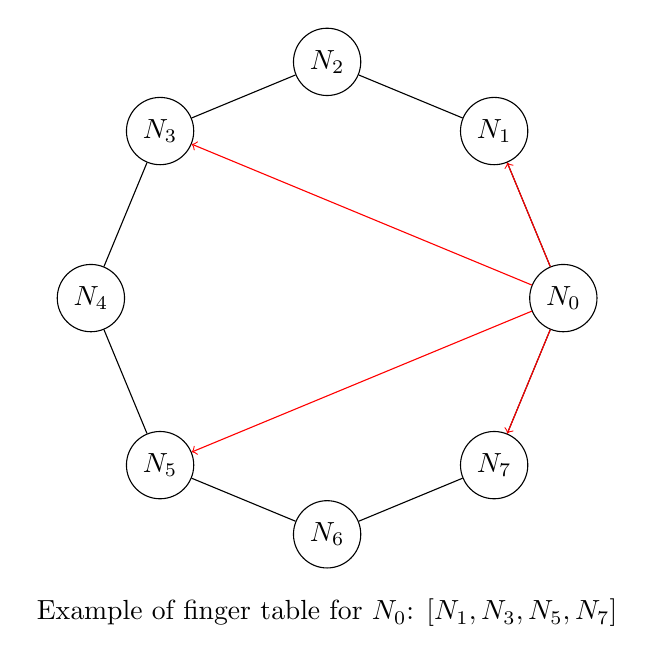
\begin{tikzpicture}
  % Nodes on the ring
  \foreach \i in {0,1,...,7} {
    \node[circle, draw, minimum size=0.8cm] (n\i) at (\i*45:3cm) {$N_\i$};
  }
  % Connections between nodes
  \foreach \i/\j in {0/1, 1/2, 2/3, 3/4, 4/5, 5/6, 6/7, 7/0} {
    \draw[-] (n\i) -- (n\j);
  }
  % Finger table connections for a sample node (N0)
  \draw[->, red] (n0) -- (n1);
  \draw[->, red] (n0) -- (n3);
  \draw[->, red] (n0) -- (n5);
  \draw[->, red] (n0) -- (n7);
  \node at (0,-4) {Example of finger table for $N_0$: [$N_1, N_3, N_5, N_7$]};
\end{tikzpicture}
\caption{BitTorrent, an example of unstructured \gls{p2p} network.}
\label{fig:BitTorrent}
\end{figure}

In this example, node $N_0$ has a finger table containing nodes $N_1, N_3, N_5$ and $N_7$.
When $N_0$ wants to find a key (representing a torrent or a peer holding pieces of a torrent), it consults its finger table to determine the closest preceding node and forwards the query until it reaches the node responsible for the key.
This ensures that the lookup operation is performed efficiently, typically within $\mathcal{O}(\log n)$ hops.
Finger tables have been mentioned in this example, without spontaneously explaining what they are and what they are used for.
A full explanation of them can be found in Section \ref{sec:finger-tables}.

\subsubsection*{Real-World Applications}
Structured \gls{p2p} systems have found application in various domains due to their efficiency and scalability.
Some notable real-world applications include \glspl{cdn}, distributed storage systems, and \gls{dns}.
Systems like BitTorrent utilize structured overlays to efficiently locate and distribute files among peers (\cite{cohen2003incentives}).
The structured approach ensures that pieces of a file can be found and downloaded quickly, even as peers join and leave the network.
Amazon's Dynamo, a highly available key-value store, leverages \glspl{dht} to manage data replication and partitioning (\cite{DeCandia2007}).
Dynamo's architecture ensures that data is evenly distributed across nodes and can be retrieved even in the presence of node failures.
The Coral \gls{cdn} uses a structured \gls{p2p} system to implement a decentralized \gls{dns} service, improving robustness and scalability (\cite{CoralCDN2010}).

\subsubsection*{Advantages and Challenges}
Structured \gls{p2p} systems offer several advantages that make them suitable for large-scale distributed applications.
The deterministic nature of \glspl{dht} ensures that data can be located within a bounded number of hops, typically $\mathcal{O}(\log n)$, where $n$ is the number of nodes in the network.
These systems can scale to accommodate a large number of nodes without significant degradation in performance.
The use of consistent hashing ensures even distribution of data and load across nodes.
Moreover, these systems are designed to handle node churn gracefully.
When nodes join or leave the network, only a small fraction of the keys need to be redistributed, minimizing disruption.

Despite their advantages, structured \gls{p2p} systems face several challenges.
Maintaining the structured overlay network requires nodes to frequently update their routing tables, especially in high-churn environments.
This can introduce overhead and complexity.
Additionally, structured \gls{p2p} systems are vulnerable to various attacks, such as Sybil attacks, where an adversary creates multiple identities to control a significant portion of the network.
Ensuring secure and trustable node identities is crucial.
Although consistent hashing helps distribute data evenly, hotspots can still occur.
Nodes with identifiers close to popular keys may experience higher loads, necessitating additional mechanisms for load balancing.

\section{Unstructured vs Strucuted \gls{p2p} Systems}
The comparison between unstructured and structured \gls{p2p} systems reveals significant differences in various aspects such as scalability, reliability, transparency and load balancing, complexity, security, data consistency, resource discovery, and performance.

Structured \gls{p2p} systems are designed with scalability in mind.
They use deterministic algorithms and \glspl{dht} to manage resources efficiently.
This allows them to grow significantly without a proportional increase in the time required to locate resources, as the lookup time typically scales logarithmically with the number of nodes in the network, denoted as \(\mathcal{O}(\log N)\).
In contrast, unstructured \gls{p2p} systems rely on techniques like flooding or random walks for resource discovery, which can lead to significant scalability issues.
As the network expands, the number of messages required to find resources increases dramatically, causing network congestion and higher latency.

Reliability is another domain where structured \gls{p2p} systems excel.
Their structured nature and the use of \glspl{dht} ensure an even distribution of data across nodes and efficient handling of node joins and departures with minimal data movement.
Additionally, redundancy and data replication in structured systems further enhance reliability.
On the other hand, unstructured \gls{p2p} systems often depend on a small subset of nodes for resource availability.
This reliance can lead to reliability problems, especially if key nodes leave the network, potentially resulting in data loss or inaccessible resources.

In terms of transparency and load balancing, structured \gls{p2p} systems offer inherent advantages.
The \gls{dht} mechanism ensures that data is evenly distributed across all nodes, preventing hotspots and ensuring uniform load distribution.
In contrast, unstructured \gls{p2p} systems lack built-in load balancing mechanisms, leading to potential performance issues.
Popular nodes or resources can become overwhelmed, causing performance degradation unless additional overlays or mechanisms are introduced.

However, structured \gls{p2p} systems come with higher complexity.
Implementing and maintaining these systems require sophisticated algorithms for consistent hashing, overlay maintenance, and efficient routing.
Regular updates to routing tables and handling edge cases add to this complexity.
Unstructured \gls{p2p} systems are simpler to implement as they do not require a predefined structure or complex routing algorithms.
Nodes can join and leave the network with minimal overhead, making these systems easier to manage, although this simplicity comes at the cost of efficiency and performance.

Security is a critical consideration in \gls{p2p} systems.
Structured \gls{p2p} systems can be more secure due to their predictable structure and the use of cryptographic techniques in \glspl{dht}.
Nonetheless, they remain vulnerable to specific attacks such as the Sybil attack, where an adversary inserts multiple nodes to disrupt the network.
Unstructured \gls{p2p} systems, due to their lack of structure, are more susceptible to security threats.
These systems are particularly vulnerable to denial-of-service attacks and the insertion of malicious nodes, which can severely disrupt resource discovery and compromise data integrity.

Data consistency is another area where structured \gls{p2p} systems perform better.
The deterministic data placement ensures that updates are consistently propagated to all replicas, maintaining data integrity.
In unstructured \gls{p2p} systems, maintaining data consistency is more challenging due to the random replication of data across nodes.
Ensuring that all replicas are updated consistently requires additional, often complex, protocols.

Resource discovery in structured \gls{p2p} systems is efficient and predictable.
The use of \glspl{dht} ensures that any resource can be located within a logarithmic number of hops, making these systems suitable for applications requiring quick and reliable resource access.
In unstructured \gls{p2p} systems, resource discovery is less efficient, as nodes typically rely on flooding or random walks, leading to high latency and incomplete searches, particularly in larger networks.

Performance is generally better in structured \gls{p2p} systems due to the efficient resource discovery and data retrieval mechanisms.
The logarithmic scaling of lookup operations ensures that performance remains acceptable even as the network grows.
Unstructured \gls{p2p} systems can suffer from poor performance due to the inefficiency of their resource discovery methods.
Extensive message passing and potential network congestion can slow down resource retrieval times significantly.

In conclusion, structured \gls{p2p} systems offer several advantages over unstructured systems, including better scalability, reliability, load balancing, and performance.
They provide efficient resource discovery and maintain data consistency effectively.
However, these benefits come at the cost of increased complexity and implementation overhead.
Unstructured \gls{p2p} systems, while simpler and easier to deploy, face significant challenges in terms of scalability, reliability, and performance, making them less suitable for large-scale applications.
The choice between structured and unstructured \gls{p2p} systems ultimately depends on the specific requirements of the application, such as the need for efficiency, reliability, and scalability.